\section{Requisitos}
\begin{frame}
  \frametitle{Requerimientos}
  {\small 
	Para este demo se necesita:
    \begin{itemize}
    \item Android Studio instalado y con los complementos adecuados descargados
    \item Dispositivo móvil físico (o  crear un dispositivo virtual con Android)
    \item \textbf{En caso de requerir una descarga, una librería o algo en particular, mencionarlo en esta selección}
    \end{itemize}

    Pasos para crear un nuevo proyecto:
    \begin{itemize}
    \item Ejecutar Android Studio (sin no hay acceso directo, abrir una terminal, cambiarse al directorio \textit{~/android-studio/bin} y teclear \textit{./studio}
    \item Una vez abierto, crear un Proyecto Nuevo seleccionando \textit{File -> New Project}
    \end{itemize}
	\begin{center}
	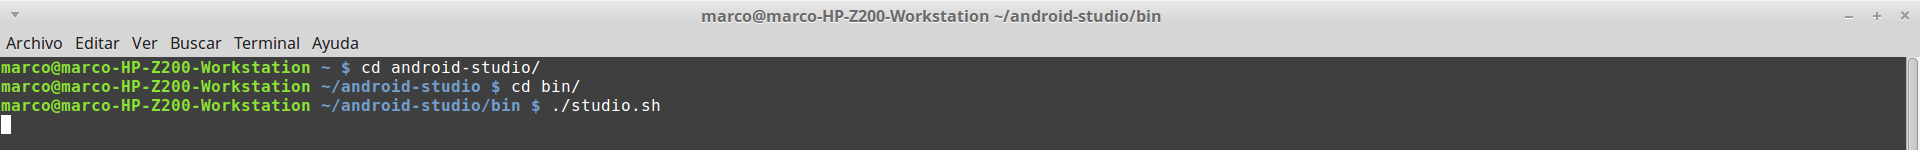
\includegraphics[height=0.75cm]{graphics/AndroidStudioSimboloSistema}
	\end{center}	
  }
  
\end{frame}

\section{Introducción}
\begin{frame}
Hablar de un FPGA, no es hablar de solo un chip más que se introdujo al área de la electrónica industrial, como pudo haber sido en sus inicios circuitos integrados (llamados ICs de aquí en adelante) con operaciones lógicas. Los FPGAs en el mundo de las simulaciones y en el prototipado, tiene un gran impacto desde hace algunas décadas. Los FPGAs las compañías de electrónicos las usan para poder generar su hardware digital, poderlo probar en una etapa temprana como los puertos de comunicación y los puertos de desarrollo que son usados durante todo el prototipado. Debido a su flexibilidad son muy requeridos en el área de la electrónica industrial. Pero vamos, ¿porqué tanto revuelo con estos circuitos integrados?. 
\end{frame}




